\section{POSIX}
\subsection{Process vs. Thread}
\begin{figure}[h!]
    \centering
    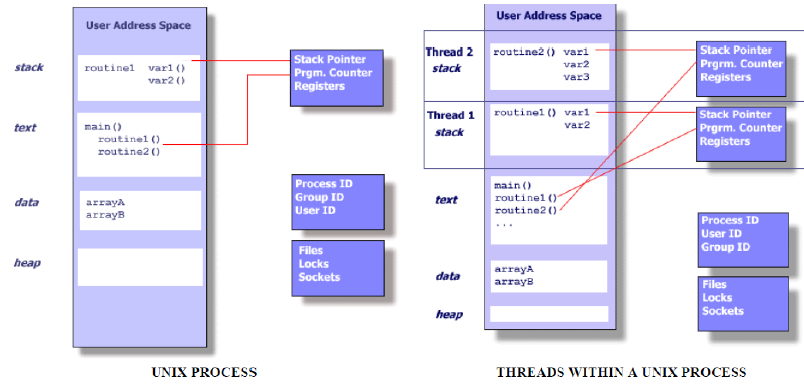
\includegraphics[width=0.8\linewidth]{images/Posix/Posix_Process_vs_Thread}
    \caption{Process vs. Thread in UNIX}
    \label{fig:posix:ProcessVsThread}
\end{figure}
\begin{itemize}
    \item Weniger Overhead und Sytemressourcen beim Erstellen und Verwalten eines Threads
    \item include pthread.h und mit link command \textbf{-lpthread} kompilieren
\end{itemize}
\subsection{Befehle}
\begin{itemize}
    \item Starten und Beenden: \textit{pthread\_create(), pthread\_exit(), pthread\_cancel()}
    \item Auf Beenden des Thrads warten: \textit{pthread\_join()}
    \item Threads Synchronisieren: \textit{ppthread\_mutex\_lock(), pthread\_mutex\_unlock()}
\end{itemize}
\subsection{Condition Variable (Mutex)}
\begin{itemize}
    \item Regelt den Zugriff unterschiedlicher Threads auf Daten
    \item Condition Variable benachrichtigt Threads beim Eintreten eines Ereignisses
    \item Gleiches Ergebnis wie mit Polling, jedoch mit kleinerer Ressourcenauslastung
\end{itemize}
\begin{figure}[h!]
    \centering
    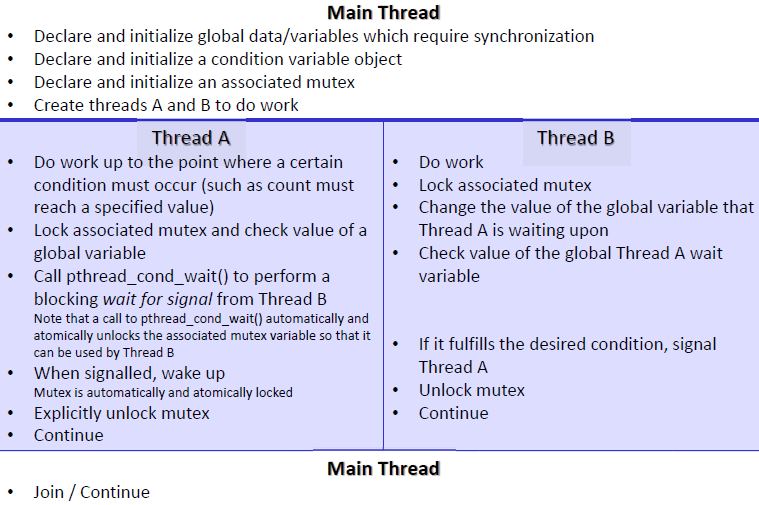
\includegraphics[width=0.5\linewidth]{images/Posix/Posix_CondVar_Sequence}
    \caption{Conditional Variable Sequence Example}
    \label{fig:posix:CondVarSequence}
\end{figure}

\subsubsection{Erstellen / Löschen}
\begin{lstlisting}[style=cpp]
int pthread_cond_init(pthread_cond_t* condVar, const pthread_condattr_t* attr);
\end{lstlisting}
\begin{lstlisting}[style=cpp]
int pthread_cond_destroy(pthread_cond_t* condVar);
\end{lstlisting}

\begin{minipage}{0.6\linewidth}
    \subsubsection{Warten}
    \begin{lstlisting}[style=cpp]
    int pthread_cond_wait(pthread_cond_t* condVar, pthread_mutex_t* mutex);
    \end{lstlisting}
    \begin{itemize}
        \item Blockiert Thread bis Signal ausgelöst wird
        \item Sollte in einer while Schleife aufgerufen werden, da allenfalls mehrere Threads auf das Signal warten
        \item Der Programmierer ist verantwortlich, die mutex wieder zu entsperren wenn der Thread fertig ist $\rightarrow$ deadlock
    \end{itemize}
\end{minipage}
\hspace{0.5cm}
\begin{minipage}{0.35\linewidth}
    \subsubsection{Signalisieren}
    \begin{lstlisting}[style=cpp]
    int pthread_cond_signal(pthread_cond_t* condVar);
    \end{lstlisting}
    \begin{itemize}
        \item Weckt den/die wartenden Threads
    \end{itemize}
\end{minipage}

\subsubsection{Variablen}
\begin{itemize}
    \item condVar: Pointer to condition variable
    \item attr: pointer to pthread\_condattr\_t structure $\rightarrow$ normalerweise 0
    \item mutex: pointer to mutex
    \item Alle Funktionen geben bei Erfolg den Wert 0 zurück
\end{itemize}

\subsection{Bounded Buffer Problem (Producer/ Consumer)}
\begin{itemize}
    \item Zwei Threads (Producer/ Consumer) teilen sich einen buffer (fixed-size)
    \item Problem: Consumer kann nichts aus einem leeren Buffer nehmen, der Producer kann nichts in einen vollen Buffer schreiben
    \item Lösung: Wenn der Buffer voll $\rightarrow$ Producer soll schlafen und wir vom Consumer benachrichtigt wenn wieder Platz vorhanden. (und umgekehrt)
    \item Dieses Problem kann mit Hilfe der Semaphoren (Mutexes), welche die inter-process/thread kommunikation ermöglicht, gelöst werden.
    \item Achtung: Darauf achten, dass die mutex Variable immer korrekt freigegeben wird $\rightarrow$ deadlock
\end{itemize}
\subsection{Beispiel (Bounded Buffer)}
\begin{multicols}{2}
    \lstinputlisting[language=C++]{code/Posix_Example.c}
\end{multicols}
